% !TeX spellcheck = sl_SI
% !TEX encoding = UTF-8 Unicode

\documentclass[a4paper, twocolumn]{article}

\usepackage[utf8]{inputenc}
\usepackage{graphicx}
\usepackage{authblk}
\usepackage[margin=22.5mm]{geometry}
\usepackage{amsmath}
\usepackage{subcaption}
\usepackage{hyperref}

\renewcommand{\figurename}{Slika}

\hypersetup{
	colorlinks=true,
	filecolor=magenta,      
	urlcolor=blue,
}

\urlstyle{same}

\begin{document}
\pagenumbering{gobble}

	\title{	\textbf{Izboljšava slik NOAA satelitov}}
	
	\author[1]{\textbf{Jan Vrhovec}}
	\affil{\textit{Univerza v Ljubljani, Fakulteta za elektrotehniko}}
	\affil[ ]{\textit{E-pošta: jv8881@student.uni-lj.si}}
	\date{}
	\maketitle
	

\section{Uvod}

Program "NOAA APT image editor" je napisan v jeziku Python z uporabo knjižnic PySide2 (grafični vmesnik), Pillow (vhodno/izhodne operacije s slikami), scikit-image (obdelava slik), numpy (matrične operacije na slikah) in matplotlib (prikaz histograma). Program je bil izdelan z namenom, da se študentom, ki bi radi sprejemali lastne vremenske slike z nizko cenovnimi SDR sprejemniki olajša naknadna obdelava in izboljšava le-teh. Namenjen je izključno slikam v formatu APT (8-bitni sivinski sliki A in B skupne širine 2080 pikslov in poljubne višine), ki ga na frekvencah okrog 137 MHz oddajajo sateliti ameriške organizacije NOAA. Program omogoča osnovno manipulacijo s slikami in različne metode izboljšave slik.


\section{Uporabljene metode izboljšav}
Izboljšava slik je dosežena z uporabo različnih metod, ki se poslužujejo matematičnih transformacij na matriki slike. Program omogoča uporabe metod kot so izravnava histograma, gama preslikava, filter mediana, ostrenje z maskiranjem, ...

\subsection{Gaussov filter}
Gaussov filter ima na sliki učinek nizko prepustnega filtra kar pomeni, da sliko zgladi in je zato primeren za odstranjevanje visokofrekvenčnega šuma. Filtriranje se izvede kot konvolucija matrike slike z filtrirnim jedrom, ki ima koeficiente izračunane po enačbi:
\begin{equation}
w(x,y)=\frac{1}{2 \pi {\sigma}^2} e^{\frac{i^2 + j^2}{2 \sigma^2}}
\end{equation}
Program omogoča, da z uporabo drsnika nastavljamo vrednost $\sigma$ in tako uravnavamo stopnjo glajenja slike.

\subsection{Gama preslikava}
Gama preslikava je uporabna takrat, kadar je kontrast slike neenakomeren pri nizkih oz. visokih sivinskih vrednostih. Za sliko z dinamičnim območjem $L$ je gama preslikava definirana po enačbi:
\begin{equation}
g(x,y)=(L-1)^{1-\gamma} f(x,y)^\gamma 
\end{equation}
\begin{figure}[]
	\centering
	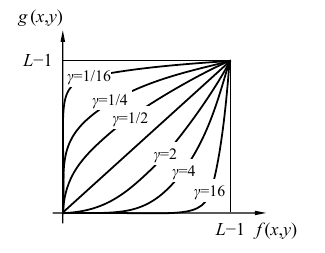
\includegraphics[width=0.8\linewidth]{gama.png}
	\caption{Oblika gama preslikave za različne vrednosti parametra $\gamma$}
\end{figure}
Program omogoča, da z uporabo drsnika nastavljamo vrednost $\gamma$. Vrednosti $\gamma>1$ povečajo kontrast svetlejših območij na račun nižjega kontrasta temnejših območij, vrednosti $\gamma<1$ pa obratno.

\subsection{Izravnava histograma}
Izravnava histograma je operacija, ki histogram slike razširi čez celotno razpoložljivo dinamično območje. To ima za posledico izboljšan kontrast slike v celotnem območju, vendar pa se kot stranski učinek poudari tudi šum. Sivinske vrednosti slike z izravnanim histogramom se določijo po enačbi:
\begin{equation}
T(s_i)=CDF(s_i) \cdot s_{max}
\end{equation}
kjer je $CDF(s_i)$ kumulativna porazdelitev slike.

\begin{figure}[h]
	\begin{subfigure}[t]{0.49\linewidth}
		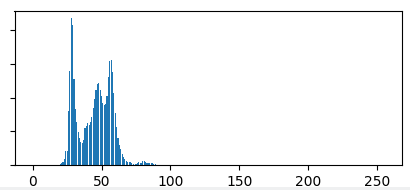
\includegraphics[width=\linewidth]{histogram_prej.png}
		\caption{Histogram slike pred izravanvo}
	\end{subfigure}
	\begin{subfigure}[t]{0.49\linewidth}
		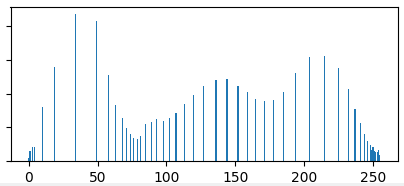
\includegraphics[width=\linewidth]{histogram_potem.png}
		\caption{Histogram slike po izravnavi}
	\end{subfigure}
	\caption{Histogram slike}
\end{figure}


\subsection{Filter mediane}
Filter mediane je operacija statističnega filtriranja, ki vsakemu pikslu slike določi novo sivinsko vrednost glede na sredinsko vrednost (mediano) pikslov v njegovi $N\times N$ okolici.
Filter mediane tako kot Gaussov filter omogoča odpravljanje šuma, vendar z občutno manj glajenja in boljšim ohranjanjem robov na sliki.

\subsection{Ostrenje z masko}
Pri ostrenju z masko najprej izračunamo masko sliko $m(x,y)$, ki je enaka razliki med prvotno sliko in zglajeno verzijo te slike:
\begin{equation}
m(x,y)=f(x,y)-F(f(x,y))
\end{equation}

Vrednost maske nato pomnožimo z faktorjem ostrenja $c$ in prištejemo prvotno sliki:
\begin{equation}
g(x,y)=f(x,y)-c \cdot m(x,y)
\end{equation}
Kot rezultat dobimo ostrejšo sliko z bolj očitnimi robovi, vendar pa se v tem procesu poudari tudi šum.

\subsection{Obarvanje slike}
Sateliti NOAA preko protokola APT oddajajo sivinske (črno-bele) slike, ki so zajete s tipali, ki so občutljivi le na eno valovno dolžino. Za sliko A je to ponavadi bližnja (0.86 $\mu m$) ali srednja IR svetloba (3.75 $\mu m$), za sliko B pa daljna IR svetloba (10.8 $\mu m$). Zaradi tega podatkov o realnih barvah slike nimamo, vendar kljub temu lahko z kombinacijo slik različnih valovnih  dolžin ustvarimo t.i. "lažne barve". Tako obarvana slika sicer nima povezave z realno barvo slikanega področja, vendar kljub temu lahko pomaga za lažje vizualno razpoznavanje tipov slikanega terena (voda, vegetacija, puščava, ...) in stanjem le-tega.\\
Program slike obarva tako, da za modri kanal barvne slike uporabi sliko B, za zeleni kanal sliko A, rdeči kanal pa se ustvari z eksponentno uteženo sliko A.

\begin{figure}[h]
	\centering
	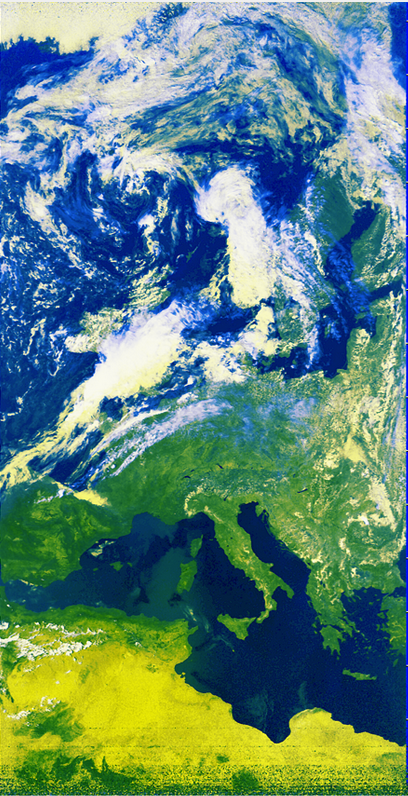
\includegraphics[width=0.4\linewidth]{false_color.png}
	\caption {Slika obarvana z lažnimi barvami}
\end{figure}


\section{Zaključek}
Program po svojih zmožnostih sicer ne ponuja nič več kot tradicionalni programi za urejanje slik, vendar pa jih prekaša v preprostosti uporabe. Uporabnik lahko z preprostim grafičnim vmesnikom hitro dostopa, do vseh metod, ki so se izkazale kot učinkovite pri izboljšanju satelitskih slik in pri tem opazuje kako se spreminja histogram slike. Kot najbolj uporabni sta se po mojem mnenju izkazali funkciji filtriranja z mediano, ki učinkovito odstrani šum in pa izravnava histograma, ki občutno popravi kontrast pri slikah z nizkim razponom sivinskih vrednosti. Zanimive rezultate pa lahko dosežemo tudi z obarvanjem slike. Prav tako se kot uporabna izkaže funkcija obračanja slike (Flip image), saj se orientacija slike spreminja glede na to ali je bil prelet satelita v času zajemanja slike v smeri sever $\rightarrow$ jug ali jug $\rightarrow$ sever.

\section{Navodila za uporabo}
Navodila za uporabo programa se skupaj z navodili za inštalacijo in pripadajočo izvorno kodo nahajajo v repozitoriju, ki je dosegljiv na naslovu:\\
\url{https://github.com/janvr1/sateliti_noaa}.

\small
\section{Viri}
\begin{enumerate}
	\item T. Vrtovec: Slikovna informatika - Laboratorijske vaje \url{http://lit.fe.uni-lj.si/gradivo/SI-LabVaje-slo.pdf}
	\item F. Mihelič, V. Štruc: Govorne in slikovne tehnologije
	\url{http://luks.fe.uni-lj.si/sl/studij/GST/pub/GST_S2a.pdf}
	\item Scikit-image dokumentacija: \url{https://scikit-image.org/docs/stable/index.html}
\end{enumerate}

	
\end{document}
